\begin{figure}[t]
\centering
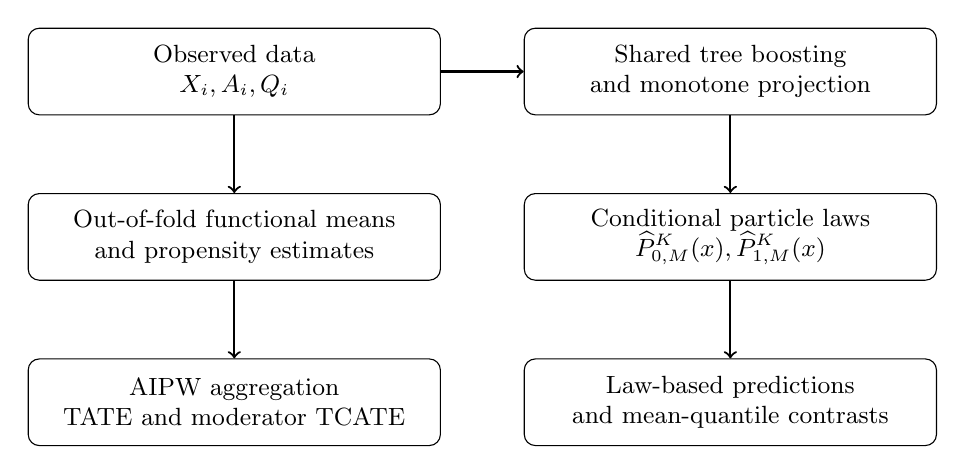
\begin{tikzpicture}[every node/.style={font=\small},box/.style={draw,rounded corners,align=center,text width=5cm,minimum height=1.1cm}]
\node[box] (data) at (0,0) {Observed data\\$X_i,A_i,Q_i$};
\node[box] (fit) at (6.3,0) {Shared tree boosting\\and monotone projection};
\node[box] (laws) at (6.3,-2.1) {Conditional particle laws\\$\widehat P_{0,M}^K(x),\widehat P_{1,M}^K(x)$};
\node[box] (nuisance) at (0,-2.1) {Out-of-fold functional means\\and propensity estimates};
\node[box] (effects) at (0,-4.2) {AIPW aggregation\\TATE and moderator TCATE};
\node[box] (lawoutputs) at (6.3,-4.2) {Law-based predictions\\and mean-quantile contrasts};
\draw[->,thick] (data) -- (fit);
\draw[->,thick] (data) -- (nuisance);
\draw[->,thick] (fit) -- (laws);
\draw[->,thick] (nuisance) -- (effects);
\draw[->,thick] (laws) -- (lawoutputs);
\end{tikzpicture}
\caption{WCF produces conditional laws and calibrated functional contrasts. The calibration uses out-of-fold particle fits and propensity estimates. It adjusts the functional contrasts without changing the final particle laws.}
\label{fig:pipeline}
\end{figure}
